\section{Inverse kinematics}\label{st:IK}
This section will show an inverse kinematics model of the CrustCrawler. The inverse kinematics model can be used to calculate the joint angles from a point in Cartesian space.

\begin{figure}[H]
    \centering
    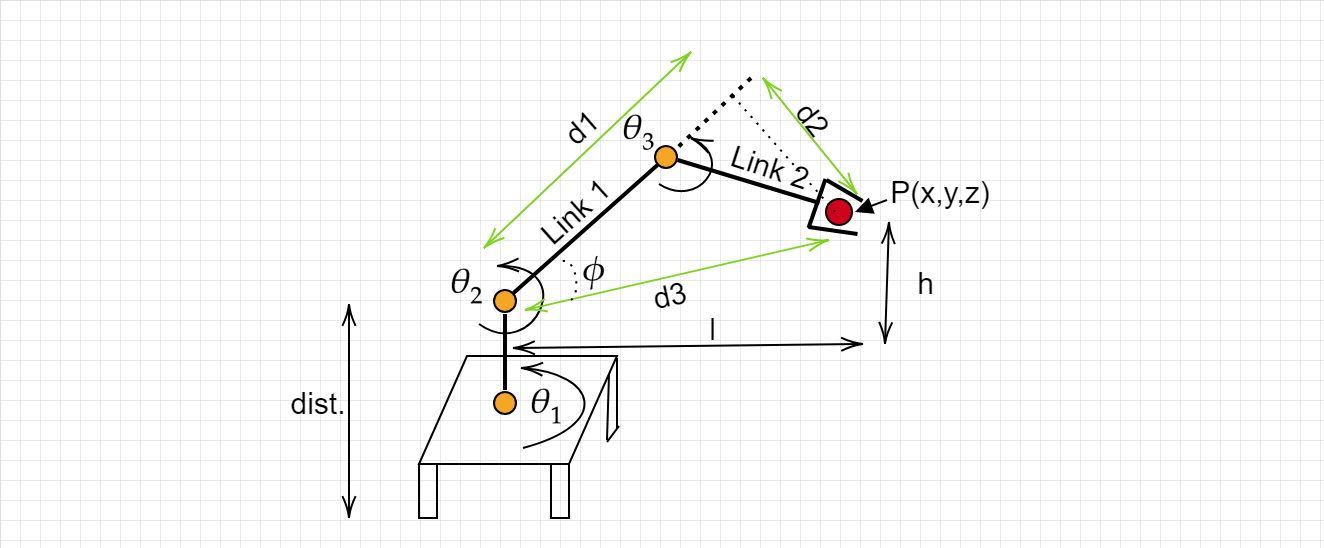
\includegraphics[width =\textwidth]{Figures/Technical_figures/invCC.png}
    \caption{Model of a 3 D.O.F manipulator, with variables visually shown}
    \label{fig:invCC}
\end{figure}
To find the angles depending on a point in Cartesian space, there is a need to isolate the variables of joint space e.i the joint angles.
In eq. \ref{eq:l} the $l$ is the projection of Link1 and Link2 onto the xy plane.
\begin{equation}\label{eq:l}
    l = \sqrt{x^2+y^2} = Link1\cdot cos(\theta_2) + Link2\cdot cos(\theta_3 - \theta_2)
\end{equation}
In eq. \ref{eq:h} the h is the projection of Link1 and Link2 onto the z axis.
\begin{equation}\label{eq:h}
    h = z - dist = Link1\cdot sin(\theta_2) - Link1\cdot sin(\theta_3 - \theta_2)
\end{equation}
The two projections in eq. \ref{eq:l} and eq. \ref{eq:h} is equal to the x,y and z - dist components. 
\begin{equation}\label{eq:equal}
    x^2+y^2+(z - dist)^2= l^2 + h^2
\end{equation}
By substitution of $l$ and $h$ in eq. \ref{eq:equal} on the right hand side, will produce a large formula, by sinus and cosine rules this could be simplified into eq. \ref{eq:expand}
\begin{equation}\label{eq:expand}
  x^2+y^2+(z - dist)^2=Link1^2+Link2^2+2 \cdot Link1 \cdot Link2 \cdot cos(\theta_3)
\end{equation} 
isolation of the cosine of $\theta_3$ is done in eq. \ref{eq:isoc3}
\begin{equation}\label{eq:isoc3}
  \frac{x^2+y^2+(z - dist)^2-Link1^2+Link2^2}{2 \cdot Link1 \cdot Link2}=cos(\theta_3)
\end{equation}
To find the symbol component of $\theta_3$, a decision have to be made elbow up, or elbow down, this is defined by the sine in front of $\theta_3$, as seen in eq. \ref{eq:elbow}.
\begin{equation}\label{eq:elbow}
    sin(\theta_3)= +\sqrt{1-cos(\theta_3)^2} \vee sin(\theta_3)= -\sqrt{1-cos(\theta_3)^2}
\end{equation}
Now the $\theta_3$ can be calculated through the use of the atan2 function, which is implemented in most mathematical tools. 
\begin{equation}\label{eq:sTheta3}
    \theta_3 = atan2(\frac{sin(\theta_3)}{cos(\theta_3)})
\end{equation}
Now that $\theta_3$ is known $\theta_2$ can be found as three variables of the triangle depicted, in green, in figure \ref{fig:invCC} is known. The green triangle is a fixed size after solving $\theta_3$, where it is located is based on the angle of $\theta_2$. In eq. \ref{eq:combi} and eq. \ref{eq:combi2} $l$ and $h$ is set to the 2 length of $d1$ and $d2$ so it is possible to solve $d3$.
\begin{equation}\label{eq:combi}
    l = \sqrt{x^2+y^2} = Link1\cdot cos(\theta_2) + Link2\cdot cos(\theta_3 - \theta_2)=d1 \cdot cos(\theta_2)+d2 \cdot sin(\theta_2)
\end{equation}
\begin{equation}\label{eq:combi2}
    h = z - dist = Link1\cdot sin(\theta_2) - Link1\cdot sin(\theta_3 - \theta_2)=d1 \cdot sin(\theta_2)-d2 \cdot cos(\theta_2)
\end{equation}
By solving for d1 and d2 in eq. \ref{eq:solvind1} and eq. \ref{eq:solvind2}, it is possible to calculate the length of d3.
\begin{equation}\label{eq:solvind1}
    d1= Link1+  Link2\cdot cos(\theta_3)
\end{equation}
\begin{equation}\label{eq:solvind2}
    d2=Link2 \cdot sin(\theta_3)
\end{equation}
Now the length d3 can be found by Pythagoras theorem in eq. \ref{eq:solvind}.
\begin{equation}\label{eq:solvind}
    d3=\sqrt{d1^2+d2^2}
\end{equation}
The angle $\phi$ is found to determine the relation between d2 and d1 by the atan2 function, as seen in eq. \ref{eq:solvinPhi}.
\begin{equation}\label{eq:solvinPhi}
    \phi= atan2(d2,d1)
\end{equation}
In eq. \ref{eq:subd1} and in eq. \ref{eq:subd2}, the cosine relation and the sinus relation, of d1 and d2, in the triangle is calculated.
\begin{equation}\label{eq:subd1}
    d1=d3 \cdot cos(\phi)
\end{equation}

\begin{equation}\label{eq:subd2}
    d2=d3 \cdot sin(\phi)
\end{equation}
Now substituting d3 in eq. \ref{eq:combi} and in eq. \ref{eq:combi2} while simplifying these, eq. \ref{eq:subdcombi} and eq. \ref{eq:subcombi2} is derived.
\begin{equation}\label{eq:subdcombi}
    l=d3 \cdot cos(\theta_2-\phi)
\end{equation}
\begin{equation}\label{eq:subcombi2}
    h=d3 \cdot sin(\theta_2-\phi)
\end{equation}
By isolating $\theta_2-\phi$ it is possible to calculate the angle of $\theta_2$, this is done in eq. \ref{eq:isothe2phi} and eq. \ref{eq:the2formel}.
\begin{equation}\label{eq:isothe2phi}
    \theta_2-\phi= atan2(h,l)
\end{equation}
\begin{equation}\label{eq:the2formel}
    \theta_2 = atan2(h,l) +atan2(d2,d1)
\end{equation}
$\theta_1$ is the relation between the x and the y coordinate, so it can be found through the tangent function.
\begin{equation}\label{eq:the1}
   \theta_1= atan2(y,x) 
\end{equation}
After calculating the final eq. \ref{eq:the1} all joint angles can be calculated from an input in a cartesian space.